The collected results give us an insight of the effect of different ISAs and \textbf{Cache} models
on performance of code execution.
\subsection{Execution Performance}
The task done by all the ISAs in consideration is same. But the way the C code is translated to
executable instruction is different in different ISAs leading different number of instructions needed to be
performed to do the same amount of job. The \texttt{simInsts} parameters from results report the number 
of simulated instructions.
\begin{figure}[h]
    \centering
    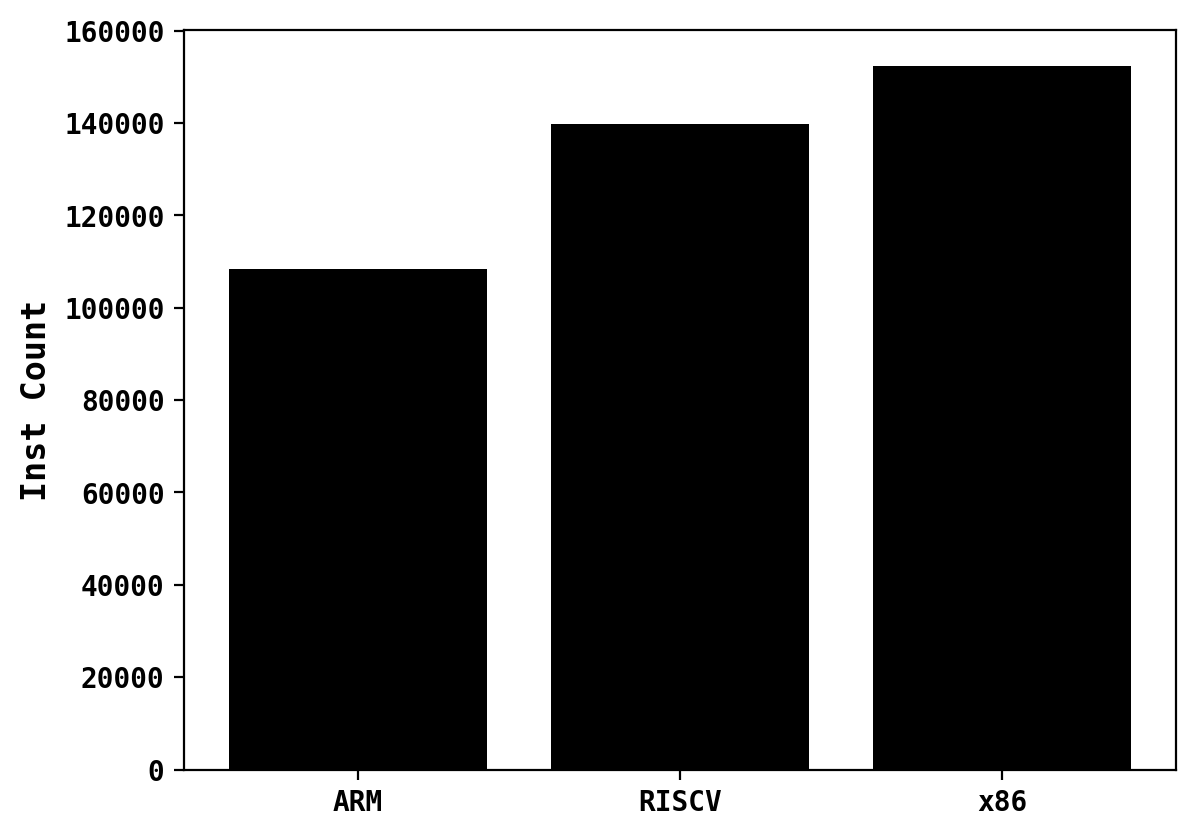
\includegraphics[width=0.8\textwidth]{./figs/1.png}
    \caption{Number of instructions executed by different architectures}
    \label{fig:Number of instructions executed by different architectures}
\end{figure}\\
From the Figure 1, we can note that \texttt{ARM} has to execute minimum number of instructions followed
by \texttt{RISCV} and \texttt{x86}. The simulation was running on a CPU with a clock frequency of
\texttt{1GHz}, implying keeping other parameters constant \texttt{ARM} will perform tasks faster compared to
the other two. This observation can be accounted to the simplicity of the instructions in \texttt{ARM}.
Unlike \texttt{x86}, \texttt{ARM} has fixed length and less number of instructions and a high code density.
Also \texttt{ARM} instructions are highly orthogonal, meaning that most instructions can work with 
any register and support various addressing modes. This reduces the need for special-purpose instructions 
and makes general-purpose ones more versatile. Although \texttt{ARM} and \texttt{RISCV} are based on same 
\texttt{RISC} principle various added advantages like conditional execution and dense addressing modes
allow for lesser instructions than \texttt{RISCV} too.\\
The trend also follows for the number of opcodes and micro-opcodes executed (\texttt{simOps}) during simulation.
\begin{figure}[h]
    \centering
    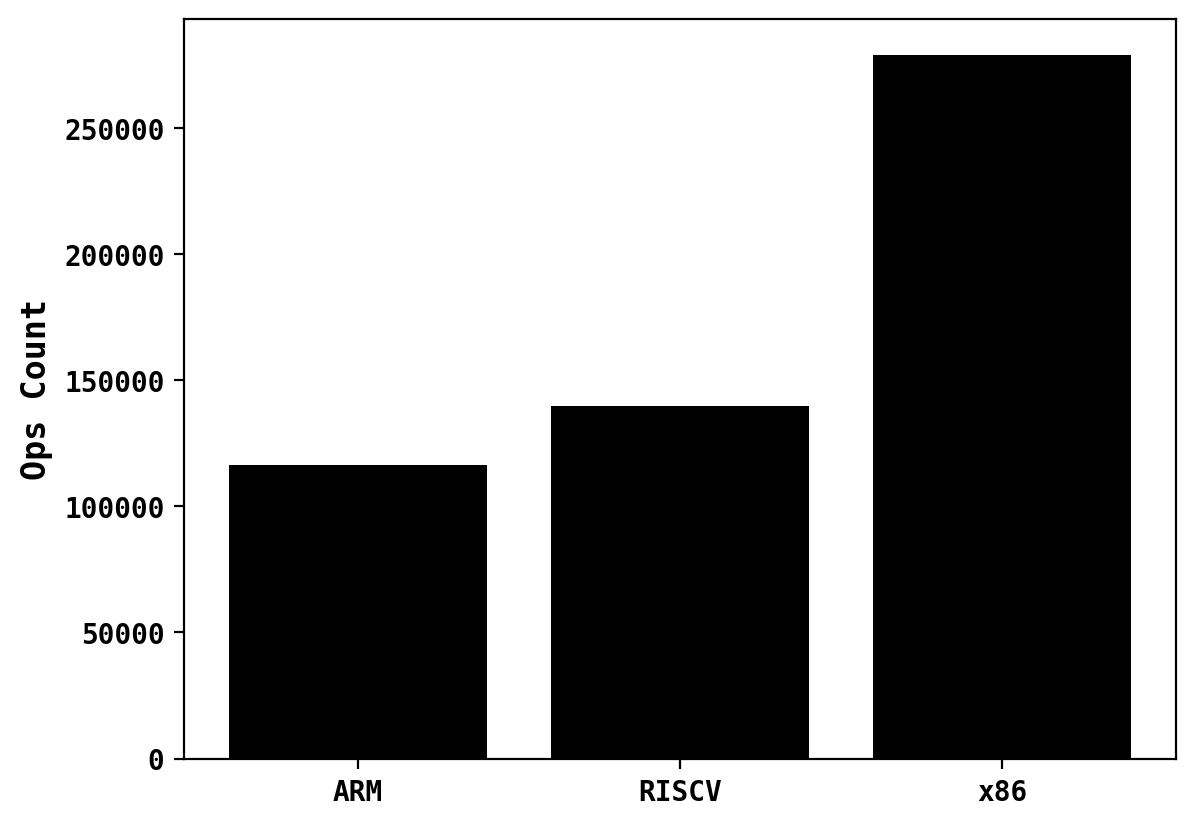
\includegraphics[width=0.8\textwidth]{./figs/2.png}
    \caption{Number of opcodes executed by different architectures}
    \label{fig:Number of opcodes executed by different architectures}
\end{figure}\\
The difference between the number of opcodes executed between \texttt{RISC} based architectures and \texttt{x86}
is stark. \texttt{x86} has to execute roughly 2.3 times more opcodes than \texttt{ARM}. Although \texttt{RISCV} is closer
to \texttt{ARM} with only 1.2 times more opcodes, highlighting the efficiency of \texttt{RISC} based programs.\\
This further translates into the runtime of the programs. From Figure 3, we can say that \texttt{ARM} perform
the task faster with a huge margin compared to others. Specifically, \texttt{ARM} took 1.8 times lesser time
to run than \texttt{x86} and 1.6 times less time than \texttt{RISCV}. Despite having a lower number of instructions
and opcodes the time of execution of \texttt{RISCV} is closer to \texttt{ARM} than \texttt{x86}. This can
be counter-intuitive to think of. But next parameter that we looked on explains this result.\\
As an instruction need not to take only one cycle to execute. In fact most
\begin{figure}[H]
    \centering
    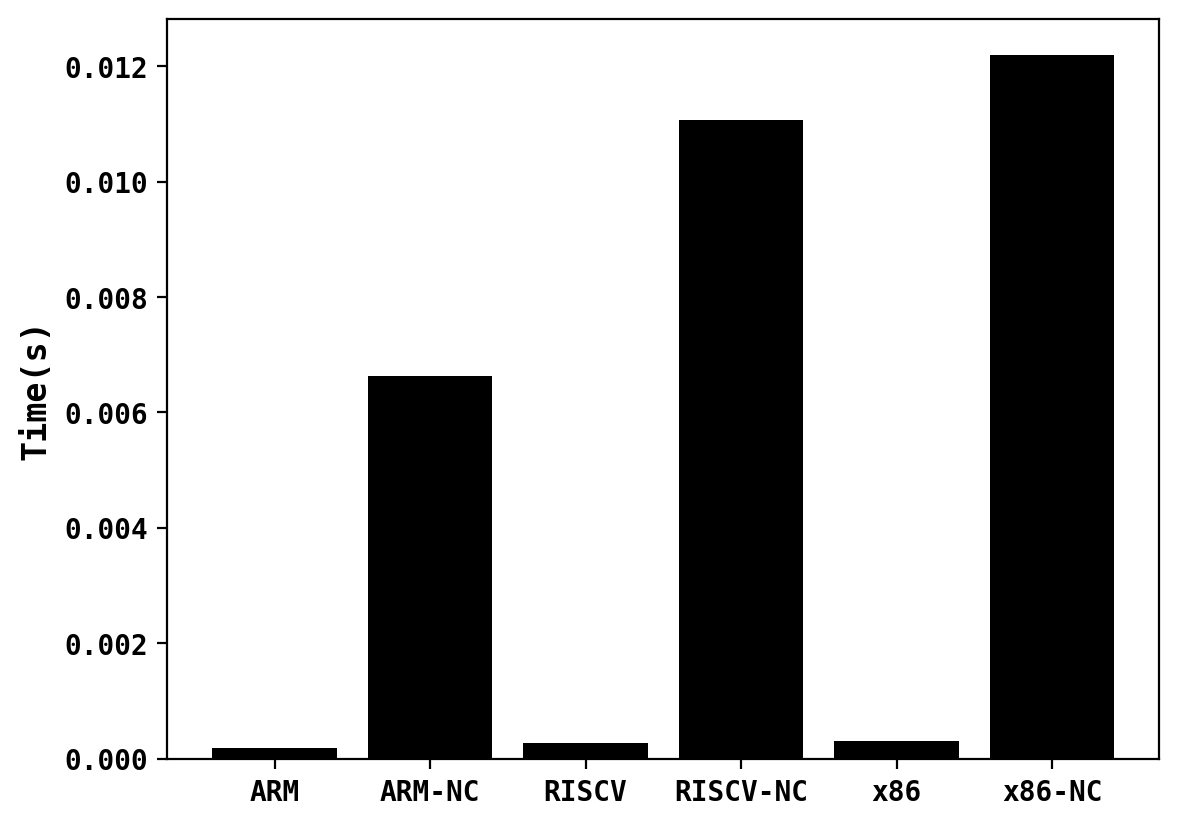
\includegraphics[width=0.8\textwidth]{./figs/3.png}
    \caption{Total execution time}
    \label{fig:Total execution time}
\end{figure}
\begin{figure}[H]
    \centering
    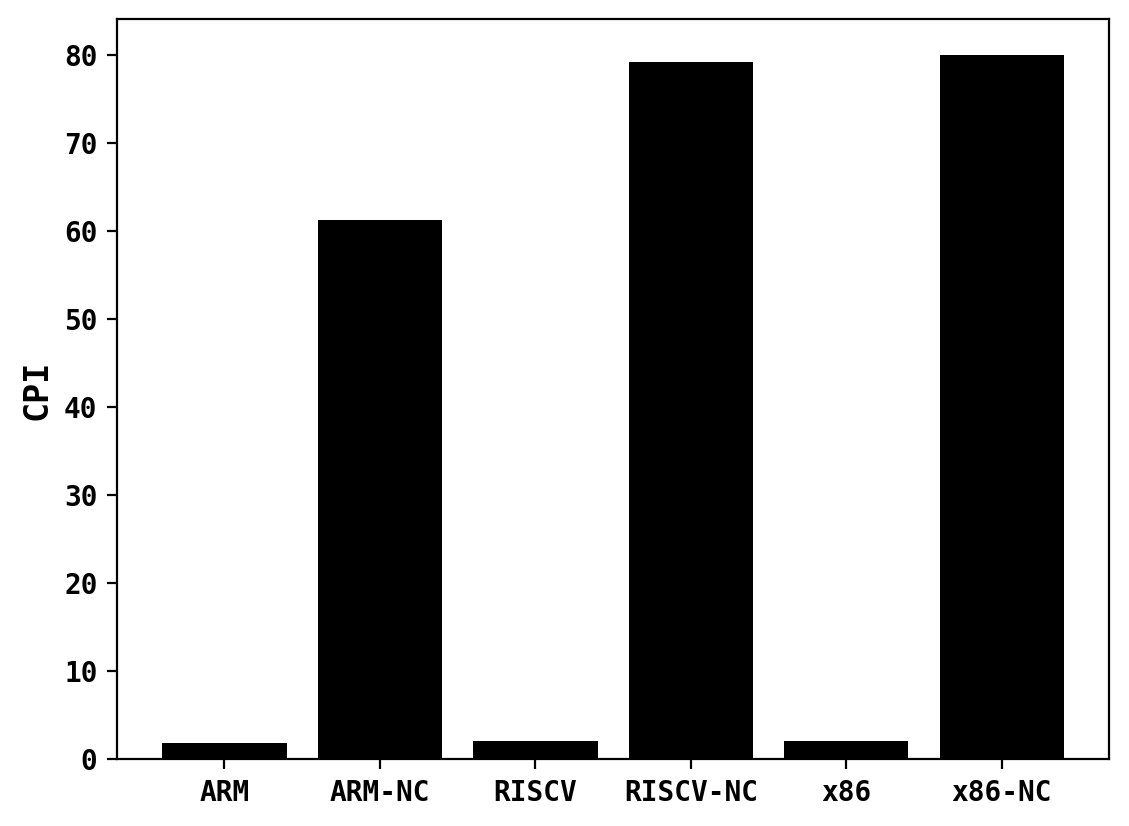
\includegraphics[width=0.8\textwidth]{./figs/4.png}
    \caption{CPI}
    \label{fig:CPI}
\end{figure}
of the instructions take multiple cycles to run. This is measured in \texttt{CPI} or cycles per 
instruction. Figure 4, shows the \texttt{CPI} of different architectures. It's evident that \texttt{RISCV}
uses more cycles to execute a single instruction compared to \texttt{ARM}. It roughly has similar \texttt{CPI}
to \texttt{x86}. Thus, \texttt{RISCV} has a larger execution time than \texttt{ARM}.\\
Overall, \texttt{ARM} performed operations faster as compared to other two mentioned accounting for lower instructions,
opcodes and a lower \texttt{CPI}. 

\subsection{Cache Performance}
\texttt{Cache} works a great deal to improve the performance of the CPU by reducing the bottle-neck of
a slower data transfer rate of the main memory. From Figure 3, the difference between the speed of \texttt{Cache}
versus \texttt{No\_Cache} system is evident. Even the fastest \texttt{ARM} without \texttt{Cache} is much slower than 
\texttt{x86} equipped with \texttt{Cache}. Taking the example of \texttt{ARM}, the \texttt{Cache} version
is roughly 35 times faster than the \texttt{No\_Cache} version of \texttt{ARM} and even \texttt{Cache} version of \texttt{x86}
is roughly 21 times faster than \texttt{No\_Cache} version of \texttt{ARM}. All other \texttt{ISAs} represent a similar
story.
\begin{figure}[H]
    \centering
    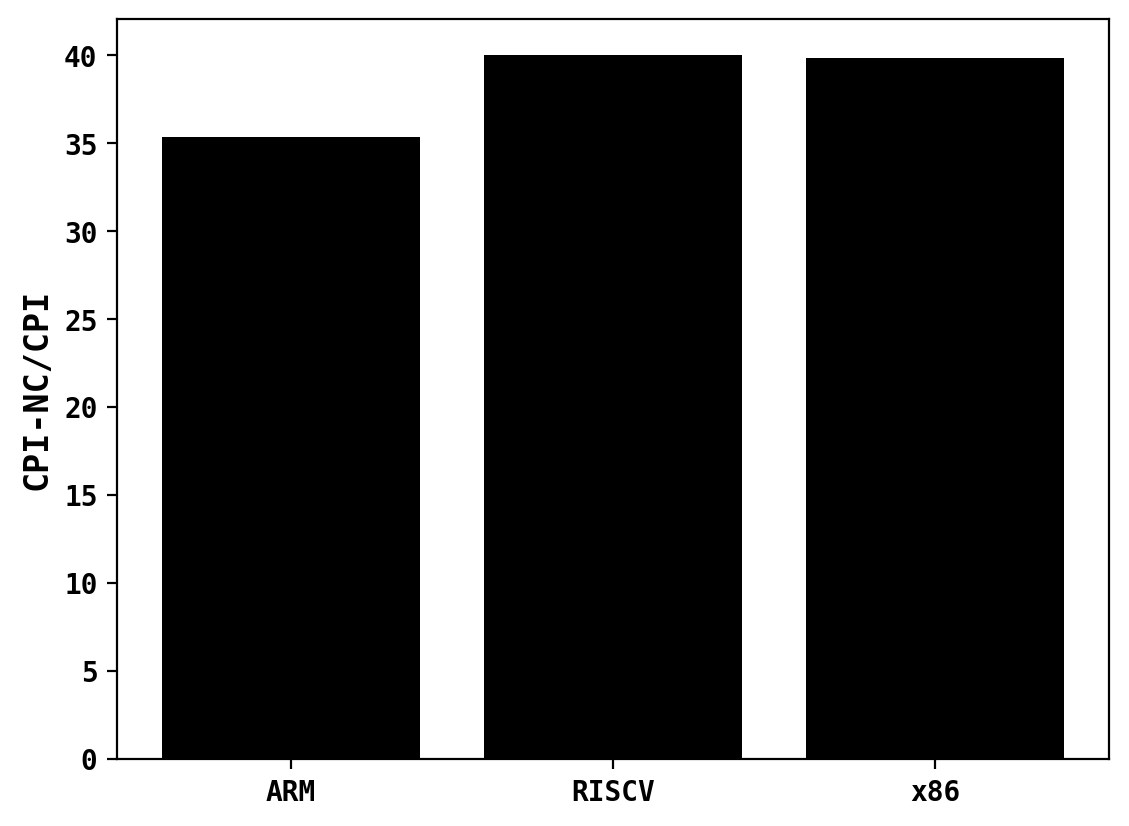
\includegraphics[width=0.8\textwidth]{./figs/5.png}
    \caption{Boost in CPI with addition of \texttt{Cache}}
    \label{fig:Boost in CPI with addition of \texttt{Cache}}
\end{figure}
From Figure 5, the addition of \texttt{Cache} has improved the \texttt{CPI} by a factor of at least 30-35.
All the previous results discussed, were done by keeping the size of problem i.e, size of sieve constant at
100. This is relatively a small problem size. To check the effect of \texttt{Cache} we can increase the problem size.
\begin{figure}[H]
    \centering
    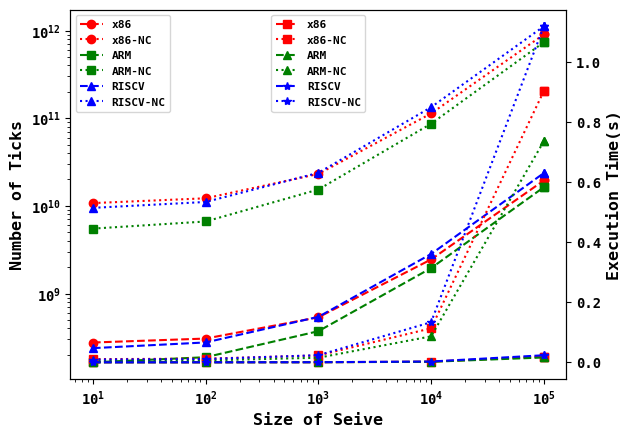
\includegraphics[width=1.0\textwidth]{./figs/6.png}
    \caption{Number of \texttt{Ticks} and execution time w.r.t size of sieve}
    \label{fig:Number of \texttt{Ticks} and execution time w.r.t size of sieve}
\end{figure}
Figure 6 shows some obvious trends that we have discussed earlier, like \texttt{No\_Cache} version are 
slower by large factor and \texttt{ARM} performs better in both \texttt{Cache} and \texttt{No\_Cache} versions
as compared to others. But new interesting observation is that \texttt{RISCV} fares slower than \texttt{x86}
for larger sizes of problem. The gap at the 1e5 between execution time of \texttt{RISCV} and \texttt{x86}
is huge.\\


The cache miss ratio is a crucial parameter in understanding the performance. Figure 7-9 show the cache miss
ratio of various \texttt{cache\_hierarchy}.
\begin{figure}[H]
    \centering
    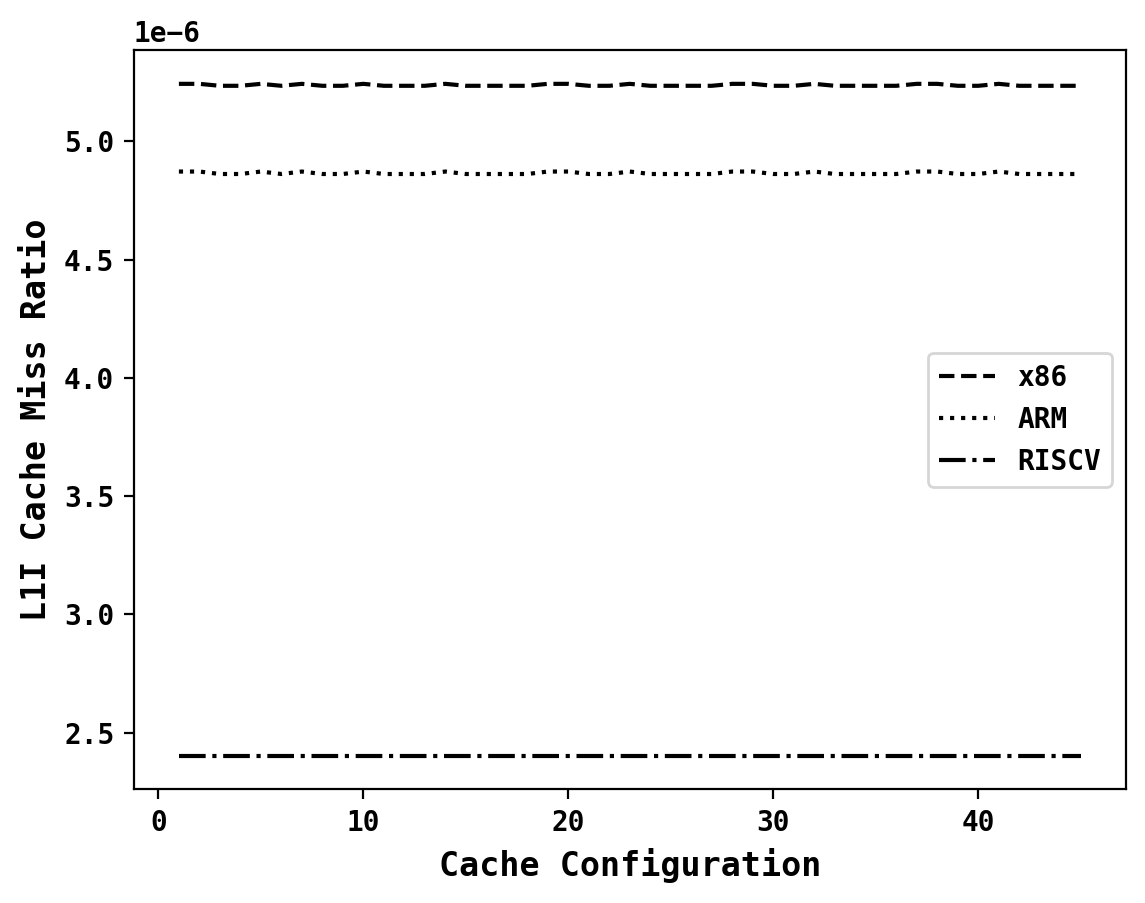
\includegraphics[width=0.8\textwidth]{./figs/8.png}
    \caption{Cache Miss ratio on L1 Instruction Cache}
    \label{fig:Cache Miss ratio on L1 Instruction Cache}
\end{figure}
\begin{figure}[H]
    \centering
    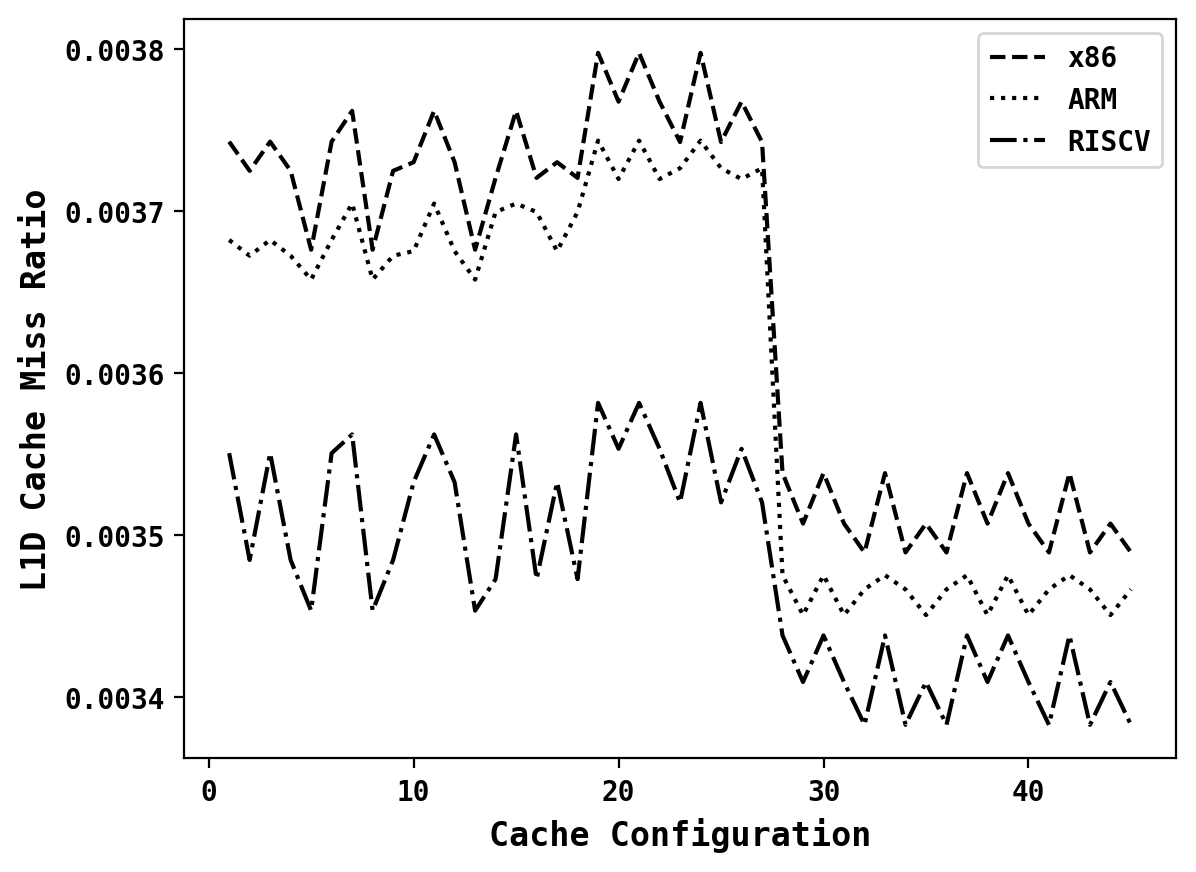
\includegraphics[width=0.8\textwidth]{./figs/7.png}
    \caption{Cache Miss ratio on L1 Data Cache}
    \label{fig:Cache Miss ratio on L1 Data Cache}
\end{figure}
\begin{figure}[H]
    \centering
    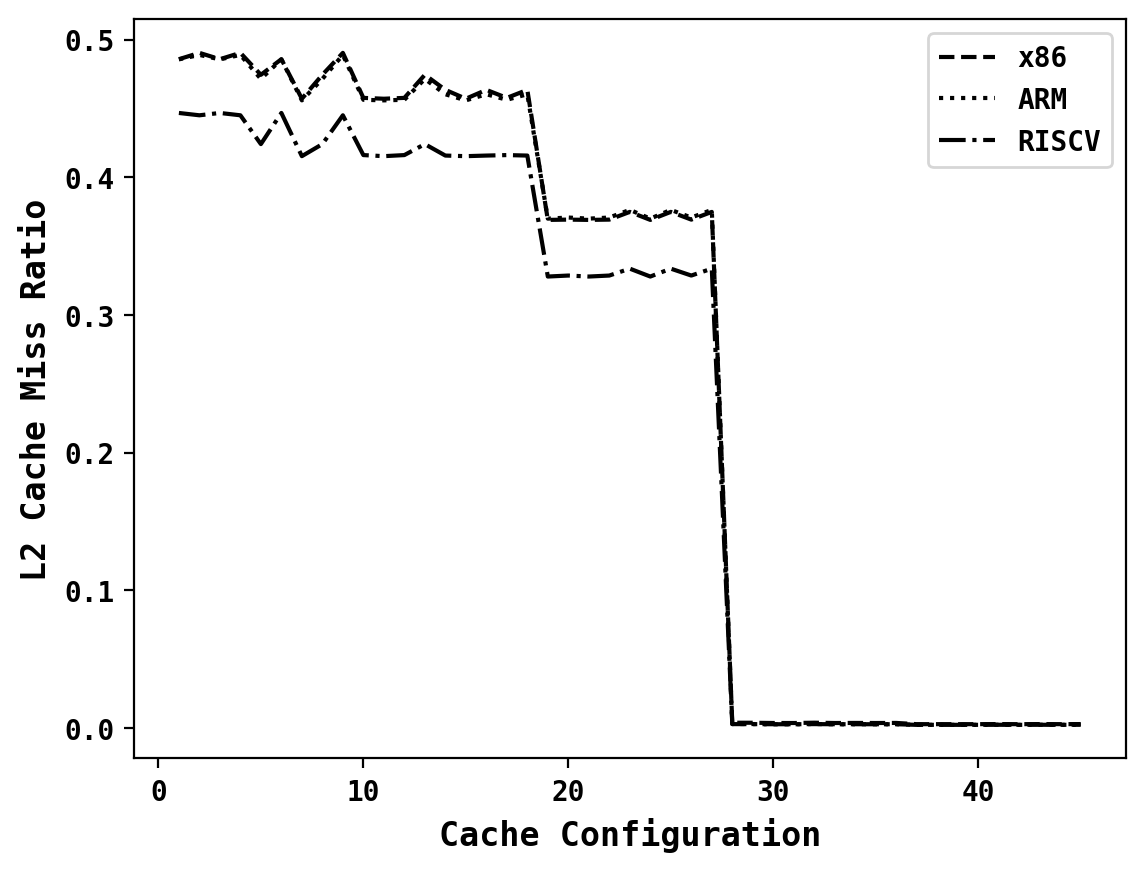
\includegraphics[width=0.8\textwidth]{./figs/9.png}
    \caption{Cache Miss ratio on L2 Cache}
    \label{fig:Cache Miss ratio on L2 Cache}
\end{figure}
From Table 2, there are three parameters affecting the \texttt{cache\_hierarchy},
namely \texttt{L1DSize}, \texttt{L1ISize} and \texttt{L2Size}. Taking the possible value from Table 2 for
each parameters we get a total of 45 configurations. The array all these configurations tuples, is then sorted
taking the sum of total cache as key. The index of these configurations in the sorted array is used to plot
the corresponding results in figures 7-9. For smaller cache sizes \texttt{ARM} and \texttt{x86} tend to perform
similar while \texttt{RISCV} performs best. This trend continues for the \texttt{L1D} cache for larger
cache sizes as well. But for \texttt{L2} cache all the architectures perform similar for larger cache sizes.\\
Figure 6 shows the cache miss ratio of the \texttt{L1I} Cache, across the architectures. Since, total number of
instructions were pretty small a larger cache size doesn't affect the miss ratio. On the other hand from Figure
8 and 9 the increase in cache size leads to significant drop in miss ratio. Specifically in case of the \texttt{L2}
cache the miss ratio drops to 0 for large cache memory. In case of the \texttt{L1D} cache the increase in
size although drops the miss ratio but that is not much significant. Major impact of the size of the cache
is seen on the \texttt{L2}'s miss ratio. Although, the effect can be attributed to the huge size increment
to \texttt{L2} from a mere \texttt{128kB} to \texttt{2048kB}. Nonetheless, all architectures perform close on
the cache miss ratio. The major factor affecting it is size not the architecture itself.